\documentclass{article}

\usepackage[utf8]{inputenc}
\usepackage[brazil]{babel}
\usepackage{amsmath, amssymb}
\usepackage{graphicx}
\usepackage{hyperref}
\usepackage{listings}
\usepackage{float}
\usepackage{xcolor}

\lstset{
    breaklines=true,
    breakatwhitespace=true,
    postbreak=\mbox{\textcolor{red}{$\hookrightarrow$}\space},
    basicstyle=\ttfamily\small,
    numbers=left,
    numberstyle=\tiny,
    stepnumber=1,
    numbersep=5pt,
    frame=single,
    showstringspaces=false,
    tabsize=4,
    language=Python
}

\title{Interferência de Ruído na Eficiência do Modelo}
\author{Eduardo Henrique Basilio de Carvalho}
\date{\today}

\begin{document}

\maketitle

\section*{Questão 1}
Seja
\begin{equation}
    H(z) = \frac{1}{z^2 + 0.2z + 0.8}
\end{equation}
\subsection*{a, b}
A figura \ref{fig:impulso_completa} mostra a resposta ao impulso, obtida pelo trecho de código \ref{lst:inicializa_e_simula_impulso}. O comportamento estável, mas oscilatório, condiz com o par de raízes $z = -0.1 \pm 0.89i$, complexas e interiores à circunferência unitária.

\begin{figure}[H]
    \centering
    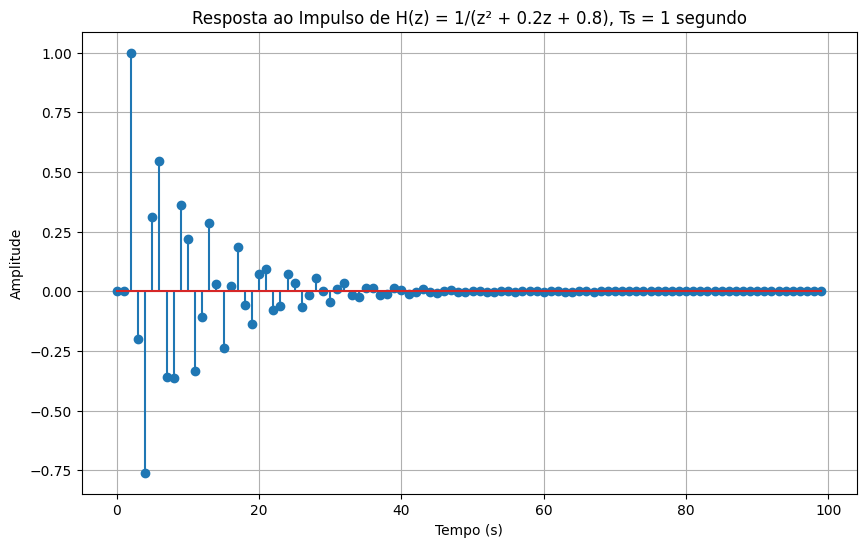
\includegraphics[width=0.8\textwidth]{imagens/impulso_completa.png}
    \caption{Resposta ao impulso do sistema}
    \label{fig:impulso_completa}
\end{figure}

\subsection*{c}
As figuras \ref{fig:impulso_transitoria} e \ref{fig:impulso_inicial} mostram um atraso puro de tempo de 2 segundos, para o tempo considerado $Ts = 1 segundo$.

\section*{Códigos}

\begin{lstlisting}[caption={Inicializa e simula resposta ao impulso}, label={lst:inicializa_e_simula_impulso}]
import numpy as np
from scipy import signal

import matplotlib.pyplot as plt

# Define the system in terms of denominator coefficients
# For H(z) = 1/(z^2 + 0.2z + 0.8), the denominator is [1, 0.2, 0.8]
num = [1]  # Numerator coefficients
den = [1, 0.2, 0.8]  # Denominator coefficients

# Set the number of samples and the sampling period
n_samples = 100
Ts = 1  # Sampling period in seconds

# Compute the impulse response
k, impulse_response = signal.dimpulse((num, den, Ts), n=100)
k, impulse_response = np.squeeze(k), np.squeeze(np.array(impulse_response))

# Plot the impulse response
plt.figure(figsize=(10, 6))
plt.stem(k * Ts, impulse_response)
plt.title("Resposta ao Impulso de H(z) = 1/(z^2 + 0.2z + 0.8), Ts = 1 segundo")
plt.xlabel("Tempo (s)")
plt.ylabel("Amplitude")
plt.grid(True)
plt.show()

# Plot the transient response
transient_t = k * Ts <= 40  # Focus on the first 40 seconds
plt.figure(figsize=(10, 6))
plt.stem(k[transient_t], impulse_response[transient_t])
plt.title("Resposta Transitoria de H(z) = 1/(z^2 + 0.2z + 0.8), Ts = 1 segundo")
plt.xlabel("Tempo (s)")
plt.ylabel("Amplitude")
plt.grid(True)
plt.show()

# Plot the start of the response, to focus on the dead time
initial_t = k * Ts <= 5  # Focus on the first 5 seconds
plt.figure(figsize=(10, 6))
plt.stem(k[initial_t], impulse_response[initial_t])
plt.title("Resposta Inicial de H(z) = 1/(z^2 + 0.2z + 0.8), Ts = 1 segundo")
plt.xlabel("Tempo (s)")
plt.ylabel("Amplitude")
plt.grid(True)
plt.show()
\end{lstlisting}

\end{document}